\documentclass[twocolumn,english]{article}
\usepackage[latin9]{inputenc}
\usepackage[landscape]{geometry}
\geometry{verbose,tmargin=0.5in,bmargin=0.75in,lmargin=0.5in,rmargin=0.5in}
\setlength{\parskip}{0bp}
\setlength{\parindent}{0pt}
\usepackage{float}
\usepackage{booktabs}
\usepackage{amstext}
\usepackage{graphicx}

\makeatletter

\providecommand{\tabularnewline}{\\}




\usepackage{array}
\usepackage{multirow}
\usepackage{amsbsy}




\providecommand{\tabularnewline}{\\}

\setlength{\columnsep}{0.25in}
\usepackage{xcolor}
\usepackage{textcomp}
\usepackage{listings}
\lstset{
  tabsize=2,
  basicstyle=\small\ttfamily,
}



\usepackage{babel}
\usepackage{listings}
\renewcommand{\lstlistingname}{Listing}

\makeatother

\usepackage{babel}
\usepackage{listings}
\renewcommand{\lstlistingname}{Listing}

\begin{document}

\title{Reference Sheet for C212 Networks and Communications}

\date{Autumn 2017}
\maketitle

\section{The Internet}

\begin{figure}[H]
\centering{}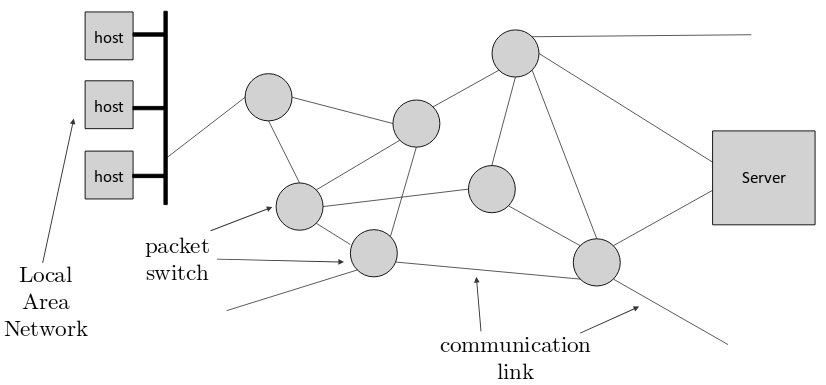
\includegraphics[width=0.75\linewidth]{img/internet}
\end{figure}

\begin{itemize}
\item \emph{Packet switch}: link-layer switch or router.
\item \emph{Communication link}: connection between packet switches and/or
end systems.
\begin{itemize}
\item Fibre optic cable, twisted pair copper wire, coaxial cable, wireless
local area links, etc.
\end{itemize}
\item \emph{Route} (\emph{path}): sequence of switches a packet goes through.
\item \emph{Protocol}: control the sending and receiving of information
between end systems/packet switches
\end{itemize}

\paragraph{Packet Switching vs Circuit Switching}

Packet-switched networks (e.g. the Internet):
\begin{enumerate}
\item Information transmitted in \emph{packets}: formatted unit of data.
\item Switches/routers operate on individual packets.
\item Switches/routers receive packets and \emph{forward} them - forwarding
decision taken on the basis of information within the packet.
\end{enumerate}
Circuit-switched networks (e.g. the telephone network):
\begin{enumerate}
\item Has a setup phase: network reserves all resources for the connection
(links, buffers, switches, etc.).
\item Links are dedicated for the entire duration of the connection.
\item Connection is destroyed and resources are freed.
\end{enumerate}
Comparing packet and circuit switching:
\begin{itemize}
\item Packet switching is \emph{connectionless}, circuit switching is \emph{connection-oriented}.
\end{itemize}
\begin{table}[H]
\centering{}%
\begin{tabular}{ccc}
\toprule 
 & \textbf{\footnotesize{}Packet Switching} & \textbf{\footnotesize{}Circuit Switching}\tabularnewline
\midrule
\emph{\footnotesize{}Setup cost} & {\footnotesize{}None} & {\footnotesize{}Expensive}\tabularnewline
\emph{\footnotesize{}Processing cost} & {\footnotesize{}For each forward} & {\footnotesize{}Little / none}\tabularnewline
\emph{\footnotesize{}Space overhead} & {\footnotesize{}For each packet} & {\footnotesize{}Little / none}\tabularnewline
\emph{\footnotesize{}Quality of Service} & {\footnotesize{}Difficult to guarantee} & {\footnotesize{}Easily guaranteed}\tabularnewline
\emph{\footnotesize{}Utilisation of links} & {\footnotesize{}Shares links - efficient} & {\footnotesize{}Limited sharing - inefficient}\tabularnewline
\bottomrule
\end{tabular}
\end{table}


\paragraph{Communication Protocols}

An agreement on how communication is to proceed.
\begin{itemize}
\item Must be an \emph{executable specification} which is \emph{unambiguous}
and \emph{complete}.
\item Needs to be able to solve \emph{addressing}, \emph{error control},
\emph{flow control}, \emph{multiplexing}/\emph{demultiplexing} and
\emph{routing}.
\end{itemize}
\begin{enumerate}
\item \emph{Handshake}: establish identities and/or contact.
\item \emph{Conversation}: exchange information.
\item \emph{Closing}: terminate conversation.
\end{enumerate}
\emph{Protocol Layering}:

\begin{figure}[H]
\centering{}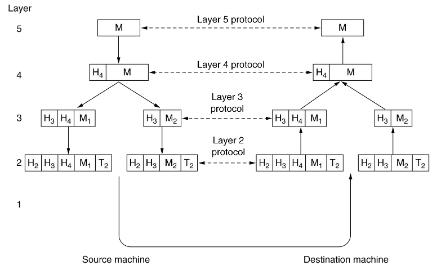
\includegraphics[width=0.5\linewidth]{img/protocol-layering}
\end{figure}

\begin{itemize}
\item \emph{Service}: set of primitives that layer provides to the layer
above.
\item \emph{Protocol}: set of rules that prescribe layout and meaning of
packets, and how the should be sent.
\item Layer $k$ puts its packet as data into a layer $k-1$ packet - which
may add a header and/or trailer.
\item \emph{Fragmentation} may be required: layer $k$ data may have to
be split accross several layer $k-1$ packets.
\end{itemize}
\emph{Internet Protocol Stack}:
\begin{enumerate}
\item \emph{Application}: defines application functionality and message
formats. E.g. Web (HTTP/HTTPS), E-mail (SMTP), BitTorrent, etc.
\item \emph{Transport}: offers connection-oriented and connectionless services.
Usually:
\begin{enumerate}
\item provides interface through \emph{sockets}, 
\item allows setting up connection, and delivering data reliably and in
the order it was sent,
\item ensures fast senders don't overwhelm slow receivers (\emph{flow control}),
\item supports \emph{secure connections}.
\end{enumerate}
\item \emph{Network (Internet)}: describes how \emph{routing} and \emph{congestion}
is solved.
\item \emph{Data Link}: allows computers to share common channel and detects
transmission errors (e.g. parity bit, checksum). E.g. Ethernet.
\item \emph{Physical}: describes transmissions of raw bits.
\end{enumerate}

\paragraph{Data Transfer}
\begin{itemize}
\item \emph{Bandwidth}: amount of information that can enter (or leave)
a connection per time unit.
\item \emph{Throughput}: actual amount of information that enters (or leaves)
connection per time unit.
\item \emph{Latency}: time it takes for one bit to go through the connection.
\item \emph{Transfer time}, $\Delta$ $=$ propagation delay (latency),
$d$ $+$ transmission delay (packet size, $L$ $/$ throughput, $R$).
\end{itemize}
With two hops, we also include \emph{router delay}, $d_{x}$, which
is made up of:
\begin{enumerate}
\item \emph{Processing delay}, $d_{\text{proc}}$: check bit errors, determine
output link (usually negligible).
\item \emph{Queuing delay}, $d_{q}$: time waiting at output link for transmission
(depends on average packet arrival rate, $a$):
\begin{enumerate}
\item $\frac{La}{R}\approx0$: small avg. queuing delay.
\item $\frac{La}{R}\rightarrow1$: large avg. queuing delay.
\item $\frac{La}{R}>1$: avg. queuing delay is infinite.
\end{enumerate}
\end{enumerate}

\section{Application Layer}

\emph{Hosts and Processes}:
\begin{itemize}
\item \emph{Host} (end system): May run multiple processes.
\item \emph{Process}: Addressed within its host by a port number.
\item \emph{Socket}: Network interface, managed by OS.
\end{itemize}
\emph{Clients and Servers}:
\begin{itemize}
\item \emph{Client}: process that initiates the communication (and establishes
connection on a connection-oriented service).
\begin{itemize}
\item Creates a socket $C$ by connecting to a server application on host
$H$ and port $P$.
\item Uses $C$ by reading and writing data into it.
\item Disconnects and destroys $C$.
\end{itemize}
\item \emph{Server}: process that waits to be contacted.
\begin{itemize}
\item Creates a socket $S$ by accepting a connection on port $P$.
\item Uses socket $S$ by reading and writing data into it.
\item Disconnects and destroys $S$.
\end{itemize}
\item \emph{Peer-to-Peer}: Processes can act as both clients and servers.
\end{itemize}

\subsection{Web (HTTP)}
\begin{itemize}
\item Uses connection-oriented transport, TCP. (port 80).
\item Consists of a sequence of requests issued by the client, and respoonses
issued by the server.
\item Stateless.
\end{itemize}

\paragraph{Requests}
\begin{enumerate}
\item Request line: \texttt{METHOD URL Protocol/Version}.
\item Header lines: \texttt{Name: Value}. 
\item Empty line.
\item Object body.
\end{enumerate}

\paragraph{Methods}
\begin{itemize}
\item \emph{GET}: retrieve object identified by URL.
\item \emph{POST}: submit data to the service.
\item \emph{OPTIONS}: request available communication options.
\item \emph{HEAD}: like GET, but without the body.
\item \emph{PUT}: store given object under given URL.
\item \emph{DELETE}: deletes given object.
\end{itemize}

\paragraph{Responses}
\begin{enumerate}
\item Status line: \texttt{Protocol/Version Code Status}.
\item Header lines: \texttt{Name: Value}.
\item Empty line.
\item Object body.
\end{enumerate}

\paragraph{Status Codes}
\begin{itemize}
\item \emph{1xx}: Informational.
\item \emph{2xx}: Successful operation.
\item \emph{3xx}: Redirection.
\item \emph{4xx}: Client error.
\item \emph{5xx}: Server error.
\end{itemize}
E.g. You can use \texttt{telnet} to make a request:

\begin{lstlisting}
telnet www.doc.ic.ac.uk 80
GET /~js4416/index.html HTTP/1.1
Host: www.doc.ic.ac.uk
\end{lstlisting}

and get a response:

\begin{lstlisting}
HTTP/1.1 200 OK
Date: ...
(Header lines) ...
Via: ...

<!DOCTYPE html>
(Page content) ...
\end{lstlisting}


\paragraph{TCP connections}
\begin{itemize}
\item HTTP/1.0 used one TCP connection per object. Now possible with \texttt{Connection: close}.
\item HTTP/1.1 introduced persistent connections - the same connection may
be used to issues multiple requests and replies.
\end{itemize}

\paragraph{Web Caching}

Improves performance and security, but adds complexity and may reduce
data `freshness'.

A client request goes to a proxy (\emph{cache}) server, which may:
\begin{enumerate}
\item Forward the request to the origin server.
\item Get the response from the origin server.
\item Store the object for some time.
\item Forward the response back to the client.
\end{enumerate}
or
\begin{enumerate}
\item Respond immediately, using a cached object.
\end{enumerate}
Implementation:
\begin{itemize}
\item Servers specify explicit expiration times using the \texttt{Expires}
header or setting \texttt{max-age} and \texttt{must-revalidate} in
the \texttt{Cache-Control} header.
\item A client or proxy can also use a \texttt{Cache-Control} header to
ensure they have a recent object. E.g. \texttt{Cache-Control: no-cache}
or \texttt{Cache-Control: max-age=60}.
\item A client or proxy can use a conditional \texttt{GET} with an \texttt{If-Modified-Since}
header.
\end{itemize}

\paragraph{Sessions}
\begin{itemize}
\item Server may use a \texttt{Set-Cookie} header, client may use \texttt{Cookie}
header.
\item Allows for sessions: users may be identified.
\end{itemize}

\paragraph{Dynamic Web Pages}
\begin{enumerate}
\item \emph{Common Gateway Interface}: identifies program and parameters
in URL, which builds and returns a webpage.
\item \emph{Scripting}: embedded scripts executed when page is processed
- may be server-side (e.g. PHP) or client side (e.g. JS).
\end{enumerate}

\subsection{Domain Name System}
\begin{itemize}
\item IPv4 (4 bytes) and IPv6 (16 bytes) addresses - easily processed by
routers.
\item Host names mapped to IP address by \emph{Domain Name System} (DNS).
\item Host names are within a hierarchical name space. There are 13 `root'
DNS servers that know where TLD servers are.
\item Each domain has an authoritative server, but caching used extensively.
\end{itemize}

\paragraph{DNS Query Types}
\begin{itemize}
\item A: maps host name to address.
\item NS: query for authoritative name server.
\item CNAME: query for a canonical (primary) name.
\item MX: query for mail exchange server.
\end{itemize}

\paragraph{DNS Protocol}
\begin{itemize}
\item Uses connectionless transport protocol, UDP (port 53).
\item Queries and replies have the same format.
\end{itemize}

\paragraph{Round Robin DNS}

Responds with a list of IP addresses , and order is changed to balance
load.

\paragraph{Tools}
\begin{itemize}
\item \texttt{host imperial.ac.uk} performs a simple DNS lookup.
\item \texttt{dig} is similar to \texttt{host -v}.
\item \texttt{nslookup imperial.ac.uk {[}ns0.ic.ac.uk{]}} queries nameservers,
you can use \texttt{-type=} for a certain query type, and can also
ask for an answer from a specific nameserver.
\end{itemize}

\paragraph{Content Distribution Networks}

Serve multiple copies at geographically distributed sites:
\begin{itemize}
\item \emph{Enter deep}: CDN servers deep into many access networks.
\item \emph{Bring home}: smaller number of large clusters in points of presence
near access networks.
\end{itemize}

\subsection{Electronic Mail}
\begin{itemize}
\item \emph{User agent} allows user to read, compose, reply to, send and
forward messages.
\item \emph{Mail servers}, accept messages for remote and local delivery
(using transport protocol), and allow user agents to access local
mailboxes (using access protocol).
\end{itemize}

\paragraph{SMTP}

Uses connection-oriented protocol, TCP.
\begin{enumerate}
\item Sets up TCP/IP connection between client and server (address can be
found from DNS).
\item Client requests server to accept its messages.
\item Server responds, so that client can send.
\end{enumerate}
Format:

\begin{lstlisting}
HELO jordanspooner.com
MAIL FROM: jordan@jordanspooner.com
RCPT TO: js4416@ic.ac.uk
DATA
From: Jordan Spooner <jordan@jordanspooner.com>
(Header lines) ...
Subject: Test Email

(Content)...
.
QUIT
\end{lstlisting}

Only supports 7-bit content - but extended by the \emph{Multipurpose
Internet Mail Extensions} (MIME) specification.

\paragraph{POP3}

Allows remote access, but assumes retrieved mail is deleted at the
server. This is solved by IMAP.
\end{document}
